\documentclass[tikz,margin=0mm]{standalone}

\usepackage{amsmath}

\usetikzlibrary{arrows}
\usetikzlibrary{decorations.pathreplacing}
\usetikzlibrary{shadows,fadings}
\usetikzlibrary{shadows.blur}
\usetikzlibrary{fit}
\usetikzlibrary{calc}

\tikzset{geometry/.style=thick}
\tikzset{feederElectrode/.style={fill=black!30!white, draw=black!80!white}}
\tikzset{electrolyte/.style={fill=black!10!white, draw=black!80!white}}

\begin{document}
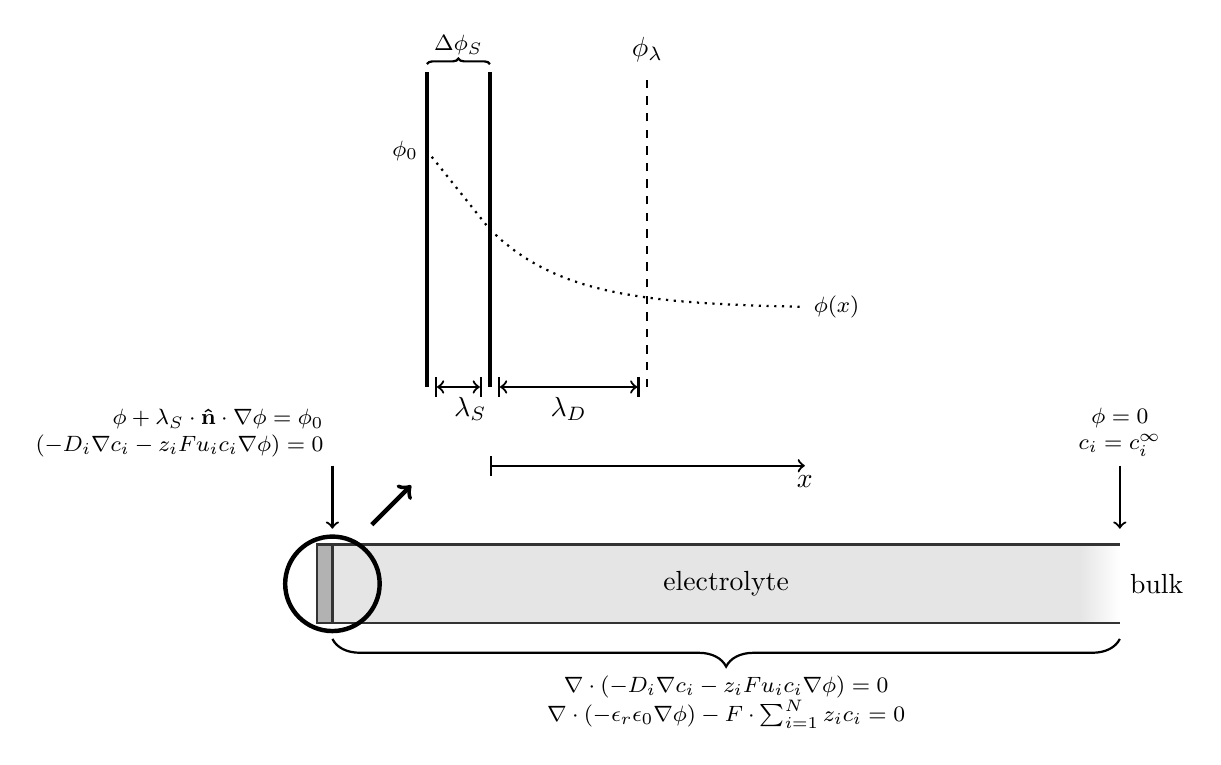
\begin{tikzpicture}[geometry]\def \sternLayerWidth{0.8}
\fill[electrolyte,draw=none] (0,0) rectangle +(10,1);
\shade[left color=black!10,right color=white,draw=none] (9.5,0) rectangle +(0.5,1);
\draw[electrolyte] (0,0) -- +(10,0) +(10,1) -- +(0,1);
\filldraw[feederElectrode] (-0.2,0) rectangle +(0.2,1);
\draw (5,0.5) node[anchor=center] {electrolyte};
\draw (10,0.5) node[anchor=west] {bulk};
\draw[ultra thick] (0,0.5) circle[,radius=0.6];
  
% electrode BC
\draw (0,2) node[node font=\footnotesize,anchor=south east,align=right] {
  	$\phi + \lambda_S \cdot \mathbf{\hat{n}} \cdot \nabla \phi = \phi_0$\\
  	$( -D_i \nabla c_i - z_i F u_i c_i \nabla \phi ) = 0$
	};
  \draw[->] (0,2) -- +(0,-0.8);
  
% bulk BC
\draw (10,2) node[node font=\footnotesize,anchor=south,align=center] {
  	$\phi = 0$\\
  	$c_i = c_i^\infty$%\\
  	%$\phi = 0$
  	};
\draw[->] (10,2) -- +(0,-0.8);
  
%% governing eq
\draw [decorate,decoration={brace,amplitude=10pt},xshift=0,yshift=0] (10,-0.2) -- +(-10,0) node [node font=\footnotesize,anchor=north,midway,yshift=-10pt,align=center]  {$ \nabla \cdot ( -D_i \nabla c_i - z_i F u_i c_i \nabla \phi ) = 0 $ \\
  	$\nabla \cdot ( - \epsilon_r \epsilon_0 \nabla \phi ) - F \cdot \sum_{i=1}^N z_i c_i  = 0$ 
  	};
\draw[->,ultra thick] (0.5,1.25) -- +(0.5,0.5);
\draw[ultra thick] (1.2,3) -- +(0,4); 
\draw[|<->|] (1.3,3) -- + (0.6,0);
\draw(1.75,3) node[anchor=north]{$\lambda_S$};
\draw[ultra thick] (2,3) -- +(0,4);
\draw[dashed] (4,3) -- + (0,4) node[anchor=south]{$\phi_\lambda$};
\draw[|->] (2,2) -- +(4,0) coordinate[label={below:$x$}] (x axis);
\draw[|<->|] (2.1,3) -- + (1.8,0);
\draw(3,3) node[anchor=north] {$\lambda_D$};
\draw[thick,dotted,domain=2:6] (1.2,6) node[node font=\footnotesize,anchor=east]{$\phi_0$} -- plot (\x, {4+exp(-(\x-2))}) node[node font=\footnotesize,anchor=west]{$\phi(x)$};
\draw [decorate,decoration={brace,amplitude=2pt},xshift=0,yshift=0] (1.2,7.1) -- +(0.8,0) node [node font=\footnotesize,anchor=south,midway,align=center]  {$\Delta \phi_S$};  
\end{tikzpicture}
\end{document}